% % % % % % % % % % % % % % % % % %
%                                 %
%  Master Thesis                  %
%  MSc in Aerospace Engineering   %
%  Mattia Gregnanin               %
%  A.Y. 2025/2026                 %
%                                 %
% % % % % % % % % % % % % % % % % %   
%                                 %
%  Main file                      %
%                                 %
% % % % % % % % % % % % % % % % % %

\documentclass[11pt]{article}

% Set paper size and margins
\usepackage[a4paper,margin={3cm,3cm}]{geometry}

% Text encoding packages
\usepackage[T1]{fontenc}
\usepackage[utf8]{inputenc}
\usepackage[english]{babel}

% Math relating packages
\usepackage{amssymb}
\usepackage{amsmath}
\usepackage{mathtools}
\usepackage{siunitx}

% Font packages
\usepackage{libertine}
\usepackage{libertinust1math}
\usepackage{bm}

% Load the xcolor package with the `rgb` option for PDF/A compatibility
\usepackage[rgb]{xcolor}

\usepackage{tikz}
\usetikzlibrary{external} % To cache figures locally
\tikzexternalize[prefix=tikz-cache/]
\usepackage{pgfplots}
\pgfplotsset{compat=1.18}
\usepgfplotslibrary{colormaps}

% Produce a PDF/A-3b
\usepackage[a-3b]{pdfx}

% For testing purposes 
\usepackage{lipsum}

\title{Master Thesis}
\author{Mattia Gregnanin}
\date{A.Y. 2025/2026}

\begin{document}
    \maketitle

    \lipsum[1]
    
    \begin{equation}
        \iint_{\partial\mathcal{V}}{\mathbf{E} \cdot d\mathbf{S}} = \iiint_{\mathcal{V}}{\frac{\rho}{\epsilon_0}d\mathcal{V}}
    \end{equation}

    \lipsum[2]

    \begin{equation}
        \begin{dcases}
            \frac{D\rho}{Dt} = - \rho\nabla \cdot \mathbf{V} \\
            \rho\frac{D\mathbf{V}}{Dt} = \rho\mathbf{g} + \nabla \cdot \bm{\mathrm{T}}
        \end{dcases}
    \end{equation}

    \lipsum[3-8]

    \begin{figure}[tp]
        \centering
        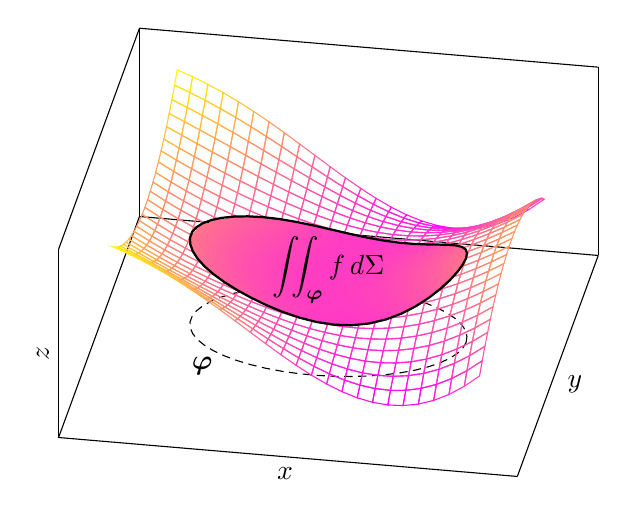
\begin{tikzpicture}
            \begin{axis}[
                xmin=-2.5,
                xmax=2.5,
                ymin=-2.5,
                ymax=2.5,
                xlabel=$x$,
                ylabel=$y$,
                zlabel=$z$,
                ticks=none,
                colormap/spring,
                view={10}{50}
            ]
                \addplot3[densely dashed,domain=0:360,samples=50,samples y=0] ({1.5*cos(x)},{sin(x)},{-4});
                \addplot3[mesh,domain=-2:2,y domain=-2:2] {x^2 - y^2*sin(deg(x))};
                \addplot3[surf,shader=interp,domain=0:360,y domain=0:1] ({1.5*y*cos(x)}, {y*sin(x)}, {2.25*y^2*cos(x)^2 - y^2*sin(x)^2*sin(deg(1.5*y*cos(x)))});
                \addplot3[thick,domain=0:360,samples=50] ({1.5*cos(x)},{sin(x)},{2.25*cos(x)^2 - sin(x)^2*sin(deg(1.5*cos(x)))});
                \node at (0,0,0.5) {$\displaystyle\iint_{\bm{\varphi}}{f\,d\Sigma}$};
                \node at (-1.2,-1,-4) {$\bm{\varphi}$};
            \end{axis}
        \end{tikzpicture}
        \caption{}
    \end{figure}
\end{document}